\section{Техническое задание}
\subsection{Основание для разработки}

Основанием для разработки является потребность в создании растрового редактора в рамках проекта по предмету "Проектирование и разработка программных систем".

\subsection{Цель и назначение разработки}

Основная цель этого проекта-разработать алгоритмические библиотеки enn используя технологии Python.

Цель разработки алгоритмической библиотеки - объединить простой и сложный лагорифмический поиск.

Задачи данной разработки включают:

\emph{для пользователя:}
\begin{itemize}
	\item используется для поиска алгоритма.
	\item позволяет отображать содержимое поляризатора.
\end{itemize}
\emph{для администратора:}
\begin{itemize}
	\item позволяет изменить режим пропуска администратора.
	\item позволяет изменять алгоритм.
	\item позволяет добавить алгоритм.
	\item используется для подавления алгоритма.
\end{itemize}

\subsection{Описание алгоритмической библиотеки}

Библиотека алгоритмов представляет собой программное обеспечение, разработанное для организации и управления набором алгоритмов. Она обладает следующими особенностями:
\begin{enumerate}
	\item \textbf{Навигация:} Доступен боковой панельный список всех алгоритмов с возможностью прокрутки, обеспечивая удобную навигацию между доступными вариантами.
	
	\item \textbf{Отображение содержимого:} Для выбранного алгоритма предоставляется область текста, где отображается его содержание с подробным описанием и примерами использования, что помогает пользователям понять его работу.
	
	\item \textbf{Режимы доступа:} Реализованы два режима доступа - пользовательский и администраторский, с обеспечением безопасности через аутентификацию по паролю для режима администратора.
	
	\item \textbf{Редактирование и управление:} Администраторы имеют возможность добавлять, редактировать и удалять алгоритмы, а также изменять пароль администратора для обеспечения полного контроля над библиотекой алгоритмов.

	
	\subsubsection{Функциональные элементы}
	Интерфейс должен предоставлять следующие элементы и функции:
	\begin{itemize}
	\item \textbf{Выбор инструментов:} Пользователи должны иметь возможность выбирать необходимые инструменты из специальной панели, обеспечивая таким образом простой и интуитивный выбор функций библиотеки.
	
	\item \textbf{Создание алгоритмов:} Должна быть возможность создавать новые алгоритмы и определять их характеристики с помощью специальных инструментов, позволяя пользователям вносить свой вклад в содержание библиотеки.
	
	\item \textbf{Редактирование алгоритмов:} Пользователи должны иметь возможность изменять существующие алгоритмы, настраивая их параметры или добавляя дополнительные функции, чтобы соответствовать их конкретным потребностям.
	
	\item \textbf{Удаление алгоритмов:} Должна быть возможность удаления нежелательных алгоритмов из библиотеки, предоставляя пользователям полный контроль над ее содержимым и качеством.
	
	\end{itemize}
	
	
	
	Композиция интерфейса редактора представлена на рисунке 2.1  и 2.2. 
	
	\begin{figure}[H]
		\centering
		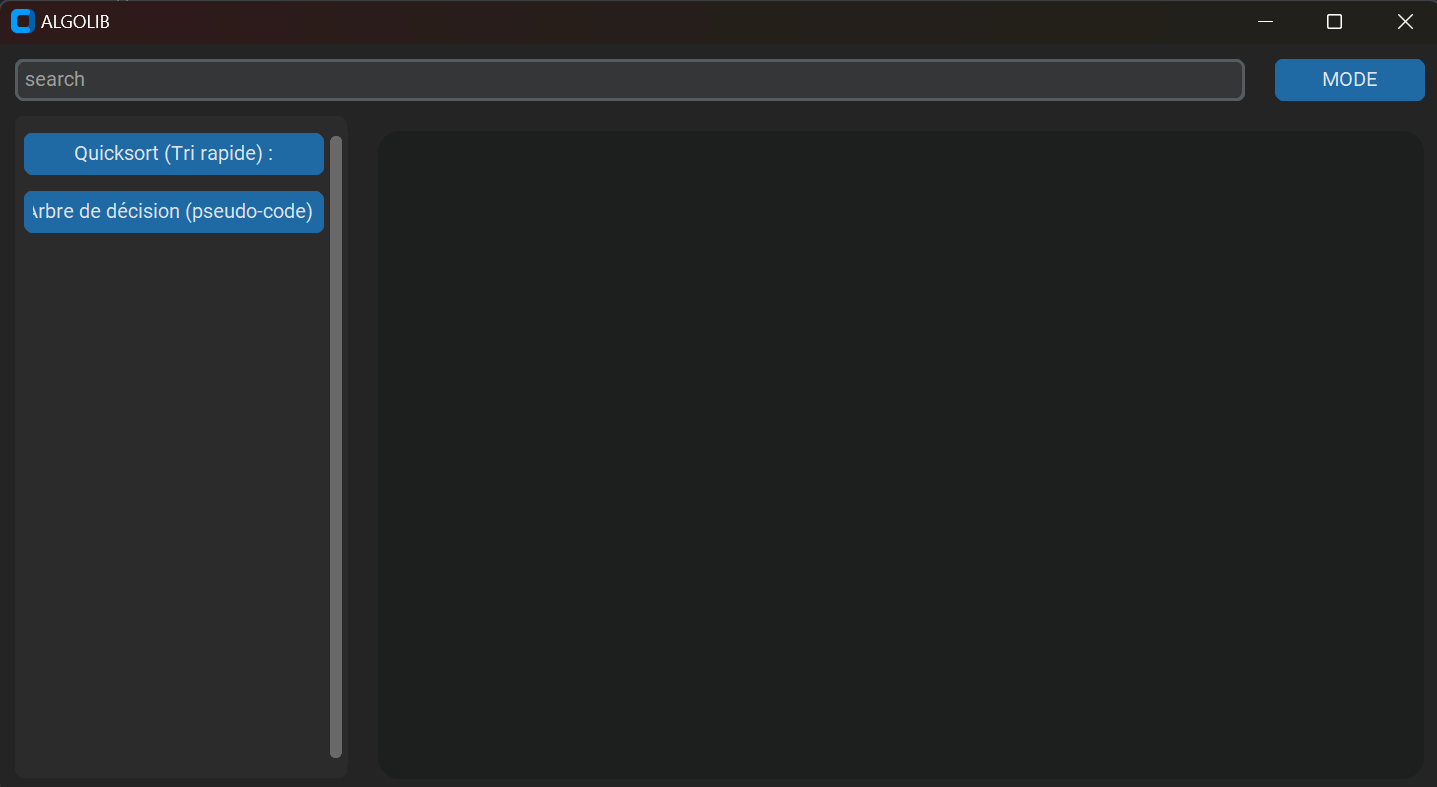
\includegraphics[width=0.7\linewidth]{images/macpaint}
		\caption{Компоновка графического интерфейса алгоритмической библиотеки.}
		\label{fig:redac_comp}
	\end{figure}

	\begin{figure}[H]
		\centering
		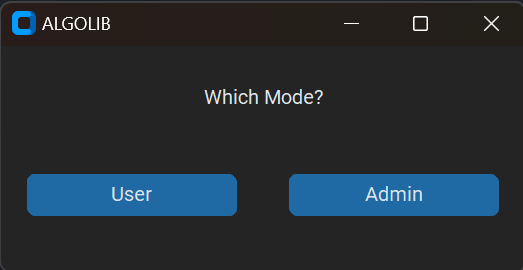
\includegraphics[width=0.7\linewidth]{images/paint}
		\caption{интерфейс с выбором из двух доступных режимов}
		\label{fig:redac_comp}
	\end{figure}
	\newpage
	
	
	
	
	
	\subsection{Требования пользователя к интерфейсу алгоритмической библиотеки}
	
	Ралгоритмическая библиотека должна создать простой и удобный интерфейс и предоставить следующие функции:
	\begin{itemize}
	\item бар поиска для фильтрации результатов по названию алгоритма.
	\item левая боковая панель с раскрывающимся списком всех алгоритмов.
	\item текстовая область с правой стороны для отображения содержимого выбранного алгоритма.
	\end{itemize}
	
	%\begin{figure}[ht]
	%\caption{Композиция шаблона сайта}
	%\label{templ:image}
	%\end{figure}
	%\vspace{-\figureaboveskip} % двойной отступ не нужен (можно использовать, если раздел заканчивается картинкой)
	
	\subsection{Моделирование вариантов использования}
	\subsubsection{Диаграмма прецедентов}
	Для библиотеки алгоритмов было разработано моделирование, позволяющее четко визуализировать различные варианты использования этой библиотеки. Это моделирование облегчает физическую разработку и подробный анализ взаимодействий между различными функциями и компонентами библиотеки. При создании этого моделирования предпочтение было отдано использованию языка визуального моделирования UML.
	
	Диаграмма вариантов использования описывает основную функциональность библиотеки алгоритмов. Это включает в себя действия, которые библиотека будет выполнять при ее использовании. Диаграмма представляет систему в виде серии вариантов использования, которые предлагаются пользователям или объектам, взаимодействующим с библиотекой. Вариант использования описывает набор действий, которые пользователь может выполнять с помощью библиотеки алгоритмов.
	
	На основе анализа функциональной области библиотеки алгоритмов необходимо реализовать следующие варианты использования :
	
	\begin{enumerate}
	\item  Поиск алгоритмов по названию.
	\item Просмотр подробной информации о конкретном алгоритме, включая его описание.
	\item Добавление новых алгоритмов в библиотеку или изменение существующих.
	\item Удаление алгоритмов из библиотеки.
	\item Обновление информации о библиотеке и ее содержимом.
	\item Изменение пароля администратора.
	\end{enumerate}
	
	
	
	\begin{figure}[ht]
		\center{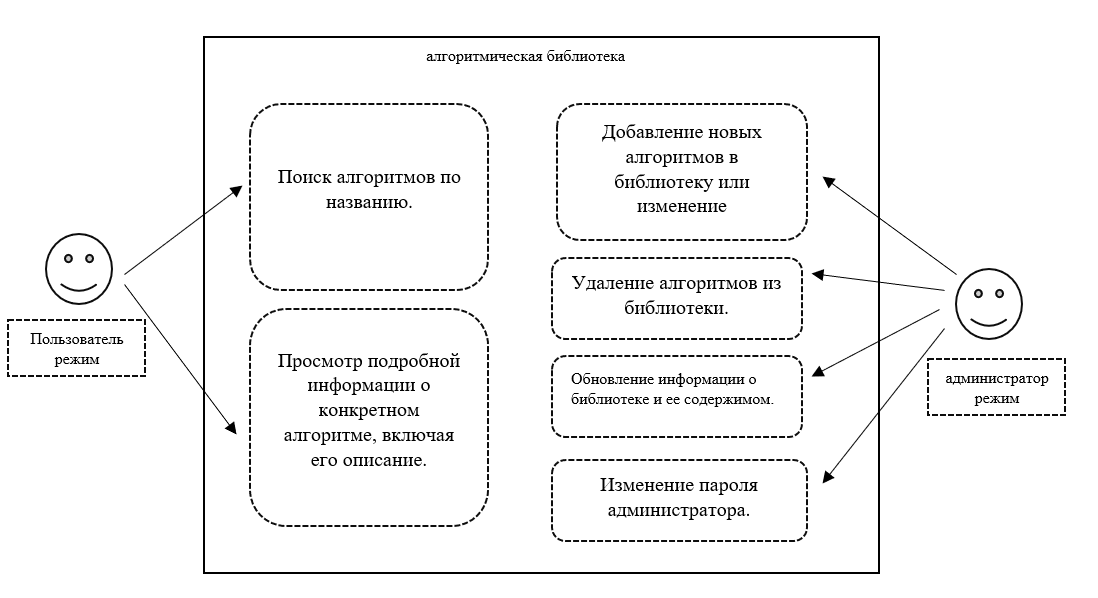
\includegraphics[width=1\linewidth]{precedent}}
		\caption{Диаграмма прецедентов}
		\label{precend:image}
	\end{figure}
	
	\subsubsection{Сценарии прецедентов программы}
	
	\begin{enumerate}
		\item Сценарий для случая использования "Поиск алгоритма":
		\begin{itemize}
			\item Основной исполнитель: Пользователь;
			\item Заинтересованные стороны и их требования: Пользователь вводит название алгоритма в строку поиска;
			\item Предварительное условие: Пользователь авторизован;
			\item Основной успешный сценарий: Алгоритм автоматически сортируется при вводе пользователем.
		\end{itemize}
		
		\item Сценарий для случая использования "Показать описание выбранного алгоритма":
		\begin{itemize}
			\item Основной исполнитель: Пользователь;
			\item Заинтересованные стороны и их требования: Пользователь должен выбрать алгоритм и отобразить его описание;
			\item Предварительное условие: Пользователь открыл библиотеку алгоритмов;
			\item Основной успешный сценарий: Пользователь нажимает на соответствующую кнопку для выбора желаемого алгоритма и отображения его описания.
		\end{itemize}
		
		\item Сценарий для случая использования "Добавить новый алгоритм":
		\begin{itemize}
			\item Основной исполнитель: Администратор;
			\item Заинтересованные стороны и их требования: Администратор должен добавить новый алгоритм в библиотеку;
			\item Предварительное условие: Администратор авторизован как администратор;
			\item Основной успешный сценарий: Администратор нажимает на кнопку "Добавить алгоритм" и следует инструкциям для успешного добавления алгоритма.
		\end{itemize}
		
		\item Сценарий для случая использования "Удалить алгоритм":
		\begin{itemize}
			\item Основной исполнитель: Администратор;
			\item Заинтересованные стороны и их требования: Администратор должен удалить существующий алгоритм из библиотеки;
			\item Предварительное условие: Администратор авторизован как администратор;
			\item Основной успешный сценарий: Администратор нажимает на кнопку "Удалить алгоритм" и следует инструкциям для успешного удаления алгоритма.
		\end{itemize}
		
		\item Сценарий для случая использования "Изменить алгоритм":
		\begin{itemize}
			\item Основной исполнитель: Администратор;
			\item Заинтересованные стороны и их требования: Администратор должен изменить существующий алгоритм в библиотеке;
			\item Предварительное условие: Администратор авторизован как администратор;
			\item Основной успешный сценарий: Администратор нажимает на кнопку "Изменить алгоритм" и следует инструкциям для успешного изменения алгоритма.
		\end{itemize}
		
		\item Сценарий для случая использования "Изменить пароль":
		\begin{itemize}
			\item Основной исполнитель: Администратор;
			\item Заинтересованные стороны и их требования: Администратор должен изменить свой пароль;
			\item Предварительное условие: Администратор авторизован как администратор;
			\item Основной успешный сценарий: Администратор нажимает на кнопку "Изменить пароль" и следует инструкциям для успешного изменения пароля.
		\end{itemize}
	\end{enumerate}
	
	\subsection{Требования к оформлению документации}
	
	Разработка программной документации и программного изделия должна производиться согласно ГОСТ 19.102-77 и ГОСТ 34.601-90. Единая система программной документации.
	